\section{Simulation de l'attaque}

Dans cette section, nous allons tenter de simuler l'attaque construite jusqu'à présent. 
Nous allons décrire les différentes étapes de l'attaque, et tenter d'anticiper les réactions
de Monsieur Astier. Finalement, nous allons énumérer les résultats qui seraient potentiellement obtenus
et ce que nous pourrions en tirer en tant qu'attaquant.

\subsection{Étapes de l'attaque}

L'attaque n'est pas très complexe, elle va principalement s'appuyer sur le courrier envoyé à Monsieur Astier :

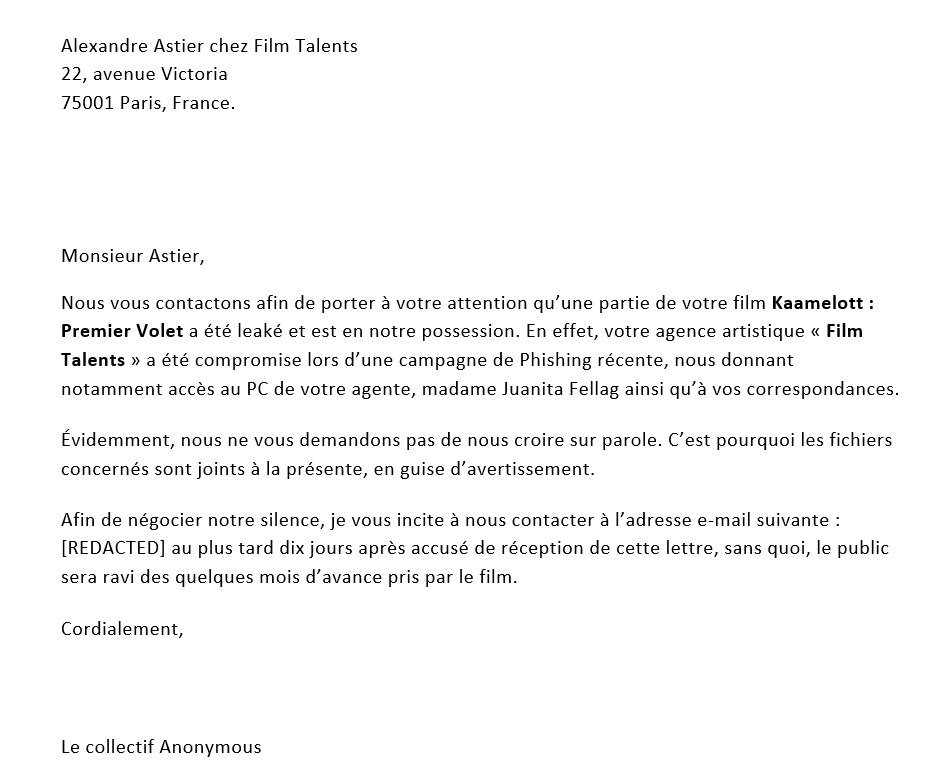
\includegraphics[scale=0.4]{images/courrier.jpeg}

Cette lettre sera envoyée avec la \textbf{Teensy}, le payload de l'attaque.
Il y a deux potentiels destinataires: Monsieur Astier et son agente artistique, Juanita Fellag. 
Nous pensons que cette lettre aboutira pour les raisons suivantes:
\begin{enumerate}
    \item Le courrier des lecteurs est systématiquement lu, et c'est un vecteur d'attaque inattendu.
    \item Le (faux) piratage impacte autant M. Astier que Mme Fellag car cette dernière est CEO de l'agence
    \item Par conséquent, cette lettre joue sur l'émotion, augmentant les chances de réussite de l'infection
    \item En utilisant un nom connu du grand public (Anonymous), nous leur permettons de mieux appréhender la menace 
\end{enumerate}

Le deuxième étape consiste en l'exploitation du payload (shell reverse TCP).
Avec ce dernier, nous pourrions exfiltrer des documents, évoluer dans le réseau de l'agence (si Mme Fellag insère la clé), ou encore installer d'autres
payload (malware, key loggers, etc.)

Nous proposons une adresse mail dans la lettre, car il est aussi possible que le payload ne fonctionne
pas, ou que la peur n'aura pas suffit à la victime pour insérer la clé. Dans ce cas, elle tentera sûrement un contact, ce qui nous permettra peut-être d'obtenir
l'adresse mail d'Alexandre Astier, nous offrant un nouveau moyen d'attaque. 
\subsection{Réaction de la victime}

Il existe donc plusieurs scénarios, que nous ne pourrons pas contrôler après l'envoi de la lettre:
\begin{enumerate}
    \item La victime utilise la clé
    \item La victime n'utilise pas la clé mais écrit un mail
    \item La victime ne fait rien
\end{enumerate}
Dans les deux premiers cas, nous obtenons quelque chose. Nous pensons qu'il est assez improbable que le troisième scénario arrive car la curiosité et la peur seront trop grandes pour
simplement ignorer la manoeuvre.

Après avoir demandé à un proche de jouer le rôle d'Astier et de son agente, il arrive aux même conclusions que nous et aurait agit
selon le premier ou deuxième scénario.

En conclusion, nous sommes satisfait de l'attaque mise en place et pensons que le taux de réussite justifie l'envoi d'un payload hardware coûtant une certaine somme d'argent.
\subsection{Résultats potentiellement obtenus}

Afin de déterminer quels types de résultats nous obtenons, nous partons du principe que l'attaque a réussi.
À l'aide d'un shell ayant les droits systèmes sur la machine, nous pourrions par exemple récupérer:
\begin{enumerate}
    \item Des logins (mot de passe Windows, keyloggers, réutilisation de password..)
    \item Des documents confidentiels (avancement de ces travaux, communication privées)
    \item De nouveaux accès (privilege escalation)
\end{enumerate}
Toutes ces ressources sont précieuses et pourraient donner beaucoup de pouvoir à un attaquant. 